%
% CHAPTER 9.- Software Engineering
%

\chapterimage{AnalyticalEngine.pdf}

\chapter{Software Engineering}
\label{chap:Software-Engineering}

{\color{red} TODO: Change chapter image}

{\color{red} TODO: Rewrite this introduction}

Our final example of how to apply the theory of nescience in practice comes from the area of software engineering. The goal of this example is to show how we can apply the concept of nescience to a problem where there are no descriptions. As I have said, what it is a description depends on the particular application at hand.

In the particular case of software engineering we want to solve two related problems. The fist one is to quantitatively measure how mature is a particular software platform. The second one is how to discover new software tests, that have not been considered by the programmers, in that way we could increase the quality of the software.

The relevance will be based on software modules and data flow, and the nescience will be based on the number of lines of code for these modules. The rationale is that very well understood task are usually coded in libraries, meanwhile not very well understood problems are usually resolved ad-hoc.

Of course, the above statement is just conjectures that need more research to be confirmed, perhaps analyzind hunderd of software project, and perhaps, performing some experiments. The goal of this chapter is to show how the theory of nescience can be applied to other areas than scientific research, not to provide a quantitative measure of software quality.

\section{Redundancy of Software}

The concept of nescience applied to software engineering allow us to measure how immature is a particular software application or platform. As it was the case for scientific research topics, if we can compress a source code, probably we do not fully understand how to solve the problem at hand. The rationale is that immature software usually contains a lot of duplicated, redundant, code; meanwhile mature software it is usually composed of generic functions and libraries that provide near optimal solutions to common problems. As a consequence, if a code contains redundant elements there must exists a better way to solve the problem.

In this section we are going to study and compare the nescience of three software platforms in the area of database management systems: SQLite, PostgreSQL and Cassandra. The first two, SQLite and PostgreSQL, are relational database management systems based on SQL, and the third one, Cassandra, is a noSQL database (knowledge of relational databases or SQL is not required to understand this chapter). SQLite and PostgreSQL platforms are based on the C programming language, meanwhile Cassandra is written in Java. The three platforms are publicly available open source software, so the reader can repeat the experiments himself.

\subsubsection*{SQLite}

SQLite\footnote{http://www.sqlite.org}, according to the description from its web home page, \emph{is an in-process library that implements a self-contained, serverless, zero-configuration, transactional SQL database engine}. Unlike other relational databases, SQLite is not based on a client-server model, instead it is composed by a highly compact library (usually less than 500 KiB) that reads and writes directly to ordinary disk files. In fact, in SQLite a complete database with its multiple tables, indices, triggers, and views, is contained in a single disk file.

Table \ref{tab:Nescience-SQLite} provides a compilation of the results of the analysis of a selection of versions of SQLite along 15 years of continuous development (first release was published in August 2000). The columns of the table represent: the version number, the number of source code lines, the size (number of bytes) of the source code, and the size (number of bytes) of the compressed version of the source code (using the Linux tool {\tt gzip}). The final column contains the nescience associated to each version.

The analysis was performed in a Linux-based machine. The command issued to compute the number of source lines of each version was:

\begin{verbatim}
# find SQLite-1_0/src -name '*.[chyl]' -exec cat {} \; > total-1.0
\end{verbatim}

\begin{table}
\begin{centering}
\begin{tabular}{|c|c|c|c|c|}
\hline 
Version & Lines & Size & Compressed & Nescience\tabularnewline
\hline
\hline
1.0 & 11,668 & 363,025 & 84,317 & 3.31 \tabularnewline
\hline
2.0 & 20,629 & 623,058 & 151,382 & 3.12 \tabularnewline
\hline
2.1 & 22,389 & 681,026 & 165,631 & 3.11 \tabularnewline
\hline
2.2 & 22,829 & 695,475 & 169,191 & 3.11 \tabularnewline
\hline
2.3 & 24,246 & 745,092 & 181,251 & 3.11 \tabularnewline
\hline
2.4 & 26,574 & 822,638 & 201,335 & 3.09 \tabularnewline
\hline
2.5 & 30,110 & 943,328 & 231,555 & 3.07 \tabularnewline
\hline
2.6 & 31,154 & 977,407 & 238,490 & 3.10 \tabularnewline
\hline
2.7 & 31,667 & 995,136 & 243,210 & 3.09 \tabularnewline
\hline
2.8 & 35,357 & 1,117,115 & 274,299 & 3.07 \tabularnewline
\hline
3.0 & 49,197 & 1,547,363 & 390,292 & 2.96 \tabularnewline
\hline
3.1 & 54,646 & 1,722,646 & 437,335 & 2.94 \tabularnewline
\hline
3.2 & 55,940 & 1,763,913 & 449,046 & 2.93 \tabularnewline
\hline
3.3 & 65,498 & 2,070,135 & 529,485 & 2.91 \tabularnewline
\hline
3.4 & 82,288 & 2,606,260 & 666,321 & 2.91 \tabularnewline
\hline
3.5 & 86,369 & 2,737,174 & 700,228 & 2.91 \tabularnewline
\hline
3.6 & 97,864 & 3,093,778 & 790,732 & 2.91 \tabularnewline
\hline
3.7 & 126,341 & 4,158,239 & 1,080,647 & 2.85 \tabularnewline
\hline
3.8 & 148,506 & 4,923,732 & 1,274,720 & 2.86 \tabularnewline
\hline
3.9 & 166,744 & 5,583,265 & 1,446,884 & 2.86 \tabularnewline
\hline
3.10 & 168,451 & 5,636,155 & 1,458,698 & 2.86 \tabularnewline
\hline
\end{tabular}
\par\end{centering}
\caption{Nescience of SQLite}
\label{tab:Nescience-SQLite}
\end{table}

Figure \ref{fig:Nescience-of-SQLite} depicts the evolution of the nescience of the SQLite platform along the different versions analyzed. As it can be observed, in general, the nescience decrease for each new release: from a nescience of 3.23 for the first, initial release, to a nescience of 2.86 in the latest published version. This behavior of nescience in SQLite is the expected behavior of a software platform that has been designed with a highly targeted goal in mind. Each new release of SQLite is focused in doing better what the software already does, instead of adding a lot of new functionality. Given the evolution of the nescience, we could say that SQLite is a software where for every new release we know better how it manage small restational databases.

\begin{figure}[h]
\centering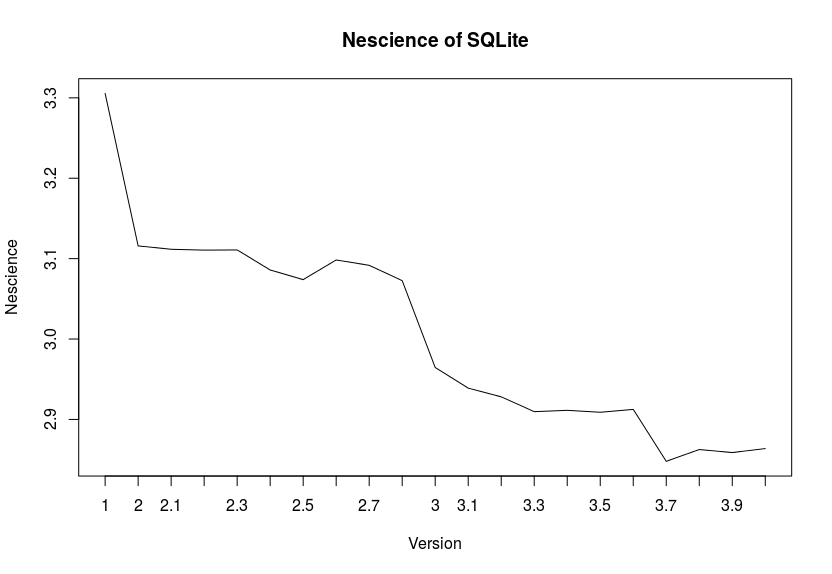
\includegraphics[scale=0.5]{SQLite_nescience}
\caption{\label{fig:Nescience-of-SQLite}Nescience of SQLite}
\end{figure}

\subsubsection*{PostgeSQL}

PostgreSQL\footnote{http://www.postgresql.org} is a full-featured open source object-relational database system, with a strong emphasis in reliability, data integrity, and correctness. PostgreSQL provides advanced database management capabilities, like tablespaces, data replication, fault tolerance, hot backups, and many others. PostgreSQL evolved from another database, the Ingres project, at the University of California, Berkeley. The team released version 1 of the new database to a small number of users in 1989, version 2 with a re-written rules system in 1990, and version 3 in 1991. After releasing version 4.2 in 1994 the project ended. All those initial releases of PostgreSQL were not included in the analysis because they are not open source. In 1996, the project was renamed to its current name PostgreSQL to reflect its support for the language SQL, and moved to an open source MIT-style license, which enabled other developers to modify and extend the source code. The first open source PostgreSQL release was version 6.0 from 1997. Currently, PostgreSQL is developed and maintained by the \emph{PostgreSQL Global Development Group}, that comprises companies and individual contributors.

Table \ref{tab:Nescience-PostgreSQL} provides a compilation of the results of the analysis of a selection of versions of PostgreSQL along 25 years of development. The columns in table have the same meaning than in Table \ref{tab:Nescience-SQLite}. The command issued to compute the number of source lines was:

\begin{verbatim}
# find postgresql-1_0/src -name '*.[chyl]' -exec cat {} \; > total-1.0
\end{verbatim}

\begin{table}
\begin{centering}
\begin{tabular}{|c|c|c|c|c|}
\hline 
Version & Lines & Size & Compressed & Nescience\tabularnewline
\hline
\hline
1.09 & 178,538 & 4,857,018 & 1,128,931 & 3.30 \tabularnewline
\hline
1.09 & 178,976 & 4,869,670 & 1,132,454 & 3.30 \tabularnewline
\hline
6.0 & 187,950 & 5,190,331 & 1,219,104 & 3.26 \tabularnewline
\hline
6.1 & 200,488 & 5,541,679 & 1,287,908 & 3.30 \tabularnewline
\hline
6.2 & 222,602 & 5,559,815 & 1,298,418 & 3.28 \tabularnewline
\hline
6.3.2 & 260,809 & 6,715,908 & 1,531,409 & 3.39 \tabularnewline
\hline
6.4.2 & 297,918 & 7,711,626 & 1,759,091 & 3.38 \tabularnewline
\hline
6.5 & 330,540 & 8,933,109 & 1,959,557 & 3.56 \tabularnewline
\hline
7.0 & 376,445 & 10,133,053 & 2,298,580 & 3.41 \tabularnewline
\hline
7.1 & 409,314 & 11,156,575 & 2,557,159 & 3.36 \tabularnewline
\hline
7.2 & 443,499 & 12,189,722 & 2,804,470 & 3.35 \tabularnewline
\hline
7.3 & 461,091 & 13,095,834 & 2,935,691 & 3.46 \tabularnewline
\hline
7.4 & 525,512 & 14,938,894 & 3,371,228 & 3.43 \tabularnewline
\hline
8.0 & 586,198 & 16,735,624 & 3,797,590 & 3.41 \tabularnewline
\hline
8.1 & 628,324 & 18,149,522 & 4,105,712 & 3.42 \tabularnewline
\hline
8.2 & 676,591 & 19,608,764 & 4,409,352 & 3.45 \tabularnewline
\hline
8.3 & 780,706 & 22,969,821 & 5,056,367 & 3.54 \tabularnewline
\hline
8.4 & 862,793 & 25,819,421 & 5,619,089 & 3.59 \tabularnewline
\hline
9.0 & 927,850 & 27,947,706 & 6,016,580 & 3.65 \tabularnewline
\hline
9.1 & 992,814 & 29,922,940 & 6,464,460 & 3.63 \tabularnewline
\hline
9.2 & 1,054,939 & 31,889,273 & 6,921,880 & 3.61 \tabularnewline
\hline
9.3 & 1,090,891 & 32,824,041 & 7,146,213 & 3.59 \tabularnewline
\hline
9.4 & 1,149,347 & 34,698,419 & 7,576,636 & 3.58 \tabularnewline
\hline
9.5 & 1,247,679 & 37,834,424 & 8,300,979 & 3.56 \tabularnewline
\hline
\end{tabular}
\par\end{centering}
\caption{\label{tab:Nescience-PostgreSQL}Nescience of PostgreSQL}
\end{table}

Figure \ref{fig:Nescience-of-PostgreSQL} depicts the evolution of the nescience of the PostgreSQL database engine along the different versions that have been published. As it can be observed, in general, the nescience increase for each new release: from a nescience of 3.30 for the first version analyzed to a nescience of 3.56 in the latest published version. This behavior of nescience in PostgreSQL is the expected behavior for a software platform that has the goal of provide as much new functionality as possible in every new release. Even if the developers have improved the already existing code, the immaturity of the new code produces an increment of the nescience of the platform. Given the evolution of the nescience, we could say that PostgreSQL is a software where for every new release it does more things but we know less about how it does them.

\begin{figure}[h]
\centering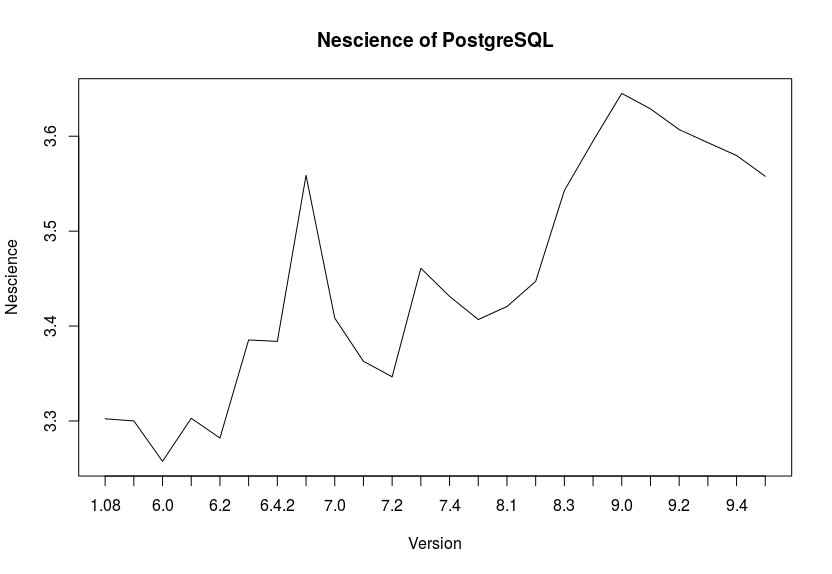
\includegraphics[scale=0.5]{PostgreSQL_nescience}
\caption{\label{fig:Nescience-of-PostgreSQL}Nescience of PostgreSQL}
\end{figure}

\subsubsection*{Cassandra}

Apache Cassandra\footnote{http://cassandra.apache.org} is an open source distributed database management system focused in scalability and high availability of data. Cassandra can provide near linear data scalability and fault-tolerance on commodity hardware. Cassandra data model is based on column indexes instead of the normalized tables of relational (SQL based) models. Cassandra was initially developed at Facebook to power their search feature, and it was released as an open source project on Google code in 2008. In 2009, it became an Apache Incubator project, and in 2010 it become a to a top-level project.

Table \ref{tab:Nescience-Cassandra} provides a compilation of the results of the analysis of a selection of version of Cassandar along 7 years of development. The columns in table have the same meaning than in Table \ref{tab:Nescience-SQLite} and Table \ref{tab:Nescience-PostgreSQL}, so the nescience of the three projects can be compared. The command issued to compute the number of source lines was:

\begin{verbatim}
# find cassandra-0.3.0/src/ -name "*.java" -exec cat {} \; > total-0.3.0
\end{verbatim}

\begin{table}
\begin{centering}
\begin{tabular}{|c|c|c|c|c|}
\hline 
Version & Lines & Size & Compressed & Nescience\tabularnewline
\hline 
\hline
0.3.0 & 50,370 & 1,747,132 & 296,565 & 4.89 \tabularnewline
\hline
0.4.2 & 35,386 & 1,217,575 & 214,303 & 4.68 \tabularnewline
\hline
0.5.1 & 36,823 & 1,286,675 & 231,918 & 4.55 \tabularnewline
\hline
0.6.13 & 39,740 & 1,402,412 & 251,556 & 4.57 \tabularnewline
\hline
0.7.10 & 64,279 & 2,321,786 & 419,346 & 4.54 \tabularnewline
\hline
0.8.10 & 77,331 & 2,764,743 & 503,978 & 4.49 \tabularnewline
\hline
1.0.12 & 88,479 & 3,152,422 & 575,984 & 4.47 \tabularnewline
\hline
1.1.12 & 106,441 & 3,857,420 & 712,932 & 4.41 \tabularnewline
\hline
1.2.19 & 142,775 & 5,240,648 & 942,257 & 4.56 \tabularnewline
\hline
2.0.16 & 165,593 & 6,177,890 & 1,105,372 & 4.59 \tabularnewline
\hline
2.1.9 & 195,424 & 7,315,659 & 1,316,190 & 4.56 \tabularnewline
\hline
2.2.1 & 212,249 & 7,928,612 & 1,399,814 & 4.66 \tabularnewline
\hline
3.0.0 & 242,320 & 9,083,317 & 1,617,120 & 4.62 \tabularnewline
\hline
\end{tabular}
\par\end{centering}
\caption{\label{tab:Nescience-Cassandra}Nescience of Cassandra}
\end{table}

Figure \ref{fig:Nescience-of-Cassandra} depicts the evolution of the nescience of the Cassandra platform along the different versions that have been analyzed. As it can be observed, the nescience presents a first period in which it clearly decreased for every release, and a second period where it increases again. A possible explanation of this behavior could be that Cassandra was a highly immature project at its initial releases (a nescience of 4.89) and during these first versions the developers improved the quality of the source code, and during the second period the developers focused more in to add new functionality.

\begin{figure}[h]
\centering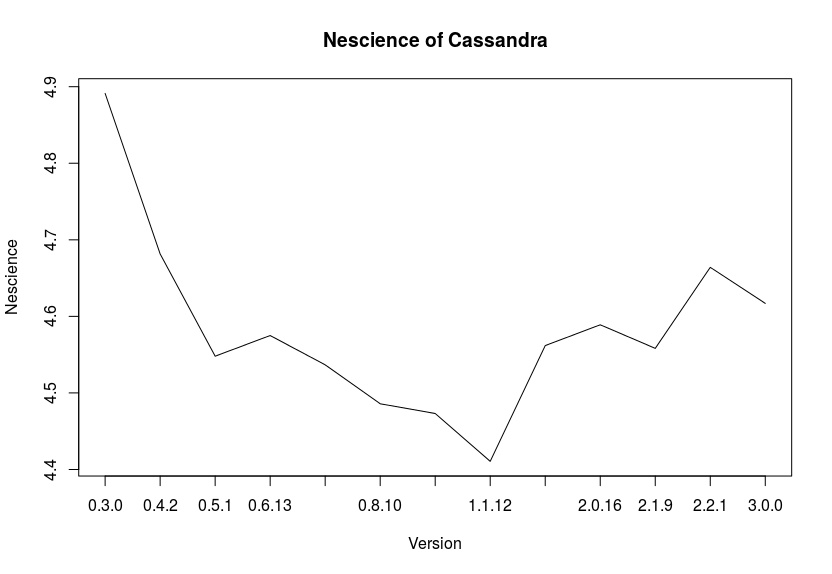
\includegraphics[scale=0.5]{Cassandra_nescience}
\caption{\label{fig:Nescience-of-Cassandra}Nescience of Cassandra}
\end{figure}

\section{Quality Assurance}

Table \ref{tab:Top-Relevance-SQLite} shows the ten most relevant functions of SQLite. The functions call graph has been computed with the aid of the cflow utility. cflow is a program that analyzes source files written in the C programming language and outputs the call graph between various functions. {\color{red} TODO: explain}

\begin{table}
\begin{centering}
\begin{tabular}{|c|c|}
\hline 
Function & Relevance \tabularnewline
\hline 
\hline
sqlite3\_free & 203 \tabularnewline
sqlite3\_malloc & 87 \tabularnewline
sqlite3\_mprintf & 69 \tabularnewline
sqlite3\_mutex\_leave & 59 \tabularnewline
sqlite3\_mutex\_enter & 57 \tabularnewline
sqlite3SafetyCheckOk & 36 \tabularnewline
fts3SqlStmt & 35 \tabularnewline
sqlite3\_realloc & 32 \tabularnewline
sqlite3\_mutex\_held & 29 \tabularnewline
sqlite3Fts3GetVarint & 20 \tabularnewline
\hline
\end{tabular}
\par\end{centering}
\caption{\label{tab:Top-Relevance-SQLite}Most relevant functions of SQLite}
\end{table}

Table \ref{tab:Top-Nescience-SQLite} shows the ten functions with higher nescience. {\color{red} TODO: explain}

\begin{table}
\begin{centering}
\begin{tabular}{|c|c|c|c|}
\hline 
Function & Description & Complexity & Nescience \tabularnewline
\hline 
\hline
fts5PorterStep4 & 3,012 & 429 & 6.02 \tabularnewline
fts5PorterStep2 & 4,101 & 600 & 5.83 \tabularnewline
sqlite3ErrName & 6,424 & 1,049 & 5.12 \tabularnewline
sqlite3ExprIfTrue & 4,015 & 988 & 3.06 \tabularnewline
winFullPathname & 5,976 & 1,475 & 3.05 \tabularnewline
unixSectorSize & 2,795 & 697 & 3.01 \tabularnewline
sqlite3GetToken & 5,967 & 1,490 & 3.00 \tabularnewline
jsonParseValue & 3,856 & 968 & 2.98 \tabularnewline
sqlite3ExprIfFalse & 5,180 & 1,301 & 2.98 \tabularnewline
sqlite3TreeViewExpr & 6,789 & 1,731 & 2.92 \tabularnewline
\hline
\end{tabular}
\par\end{centering}
\caption{\label{tab:Top-Nescience-SQLite}Highest nescience in SQLite functions}
\end{table}

Finally, Table \ref{tab:Interestingness-SQLite} shows the ten most interesting functions from the point of view of testing. {\color{red} TODO: explain}

\begin{table}
\begin{centering}
\begin{tabular}{|c|c|}
\hline 
Function & Interestingness \tabularnewline
\hline 
\hline
fts3SqlStmt & 0.55 \tabularnewline
sqlite3\_free & 0.54 \tabularnewline
sqlite3\_initialize & 0.47 \tabularnewline
sqlite3VXPrintf & 0.46 \tabularnewline
fts5CheckTransactionState & 0.43 \tabularnewline
fts5StorageGetStmt & 0.43 \tabularnewline
sqlite3Fts5GetVarint & 0.41 \tabularnewline
sqlite3TreeViewExpr & 0.38 \tabularnewline
fts5DataRead & 0.38 \tabularnewline
sqlite3Fts3SegReaderStep & 0.38 \tabularnewline
\hline
\end{tabular}
\par\end{centering}
\caption{\label{tab:Interestingness-SQLite}Interestingness of SQLite functions}
\end{table}

%
% Forex Trading Robots
%

\section{Forex Trading Robots}
\label{sec:trading}

Open source mql4 robots evaluated with metatrader4 in the EUR/USD exchange over a period of one year (2016), at intervals of five minutes, and with a fixed spread of 2 pips.
